\documentclass{beamer}

% Required Packages
\usepackage{graphicx} % Required for including images
\usepackage{babel} % Required for language settings
\usepackage{listings} % Required for code listings
\usepackage{ragged2e} % Required for text justification
\usepackage{caption}

\usefonttheme{professionalfonts}

%Theme and Color
\usetheme{Warsaw}
\usecolortheme{orchid}

% Font Sizes
\setbeamerfont{title}{size=\huge}
\setbeamerfont{frametitle}{size=\Large}

% Itemize Template
\setbeamertemplate{itemize items}[default]

% Title slide
\title{ACHIEVO}
\subtitle{A Productivity WebApp}
\institute[Program]{
	\inst{Women Engineers}
	\inst{TalentSprint}
}
\date{21/06/2023}
\begin{document}	
	\maketitle
	\begin{frame}{Team Members}
		\begin{itemize}
		\item Nidhi Iyer
		\item Khyati Satija
		\item Pankhuri Asthana
		\item Srinayana Mandalapu
		\item Anushka Shankar
		\end{itemize}
	\end{frame}

	\begin{frame}{Description}
		\begin{itemize}
		\item A user - centric web app 
		\item Focusses on the user's productivity, motivation 
		\item Salient features: pomodoro timer, to-do list, etc.
		\item Beats distractions
		\end{itemize}
	\end{frame}

	\begin{frame}{Problem Statement}
		\justifying
		\begin{itemize}
		\item Can't stay focussed for longer durations
		\item Consistency and motivation doesn't last long
		\item Hampered productivity due to social media
		\end{itemize}
	\end{frame}

	\begin{frame}{Solution}
		\justifying
		\begin{itemize}
		\item Soughts to increase the focus levels and attention span of the user
		\item It provides effective tried and tested techniques such as the Eisenhower matrix, 1-3-5 rule etc. 
		\item It acts as a virtual accountability partner and helps the user to get their tasks accomplished
		\end{itemize}
	\end{frame}
	
	\begin{frame}{Features}
                \begin{itemize}
		\item Pomodoro Technique
                \item To-Do list (1-3-5 rule)
                \item Eisenhower matrix
                \item Milestone Setting
                \item Fill the Container
                \item Reward based point system
                \item Productivity tracker
                \end{itemize}
        \end{frame}


	\begin{frame}{Future Prospects}
	\begin{columns}
        \begin{column}{0.7\textwidth} % Adjust the width as needed
            % Content on the left side of the slide
        \begin{itemize}

		\item Group and Global Leaderboards
                \item The Motivating Spinning Wheel
                \item The Good Scroll
                \item Marathon Mode
                \item The-Hour-Rule
		\item Dilemma

	\end{itemize}

        \end{column}
        
        \begin{column}{0.3\textwidth} % Adjust the width as needed
            \begin{figure}
                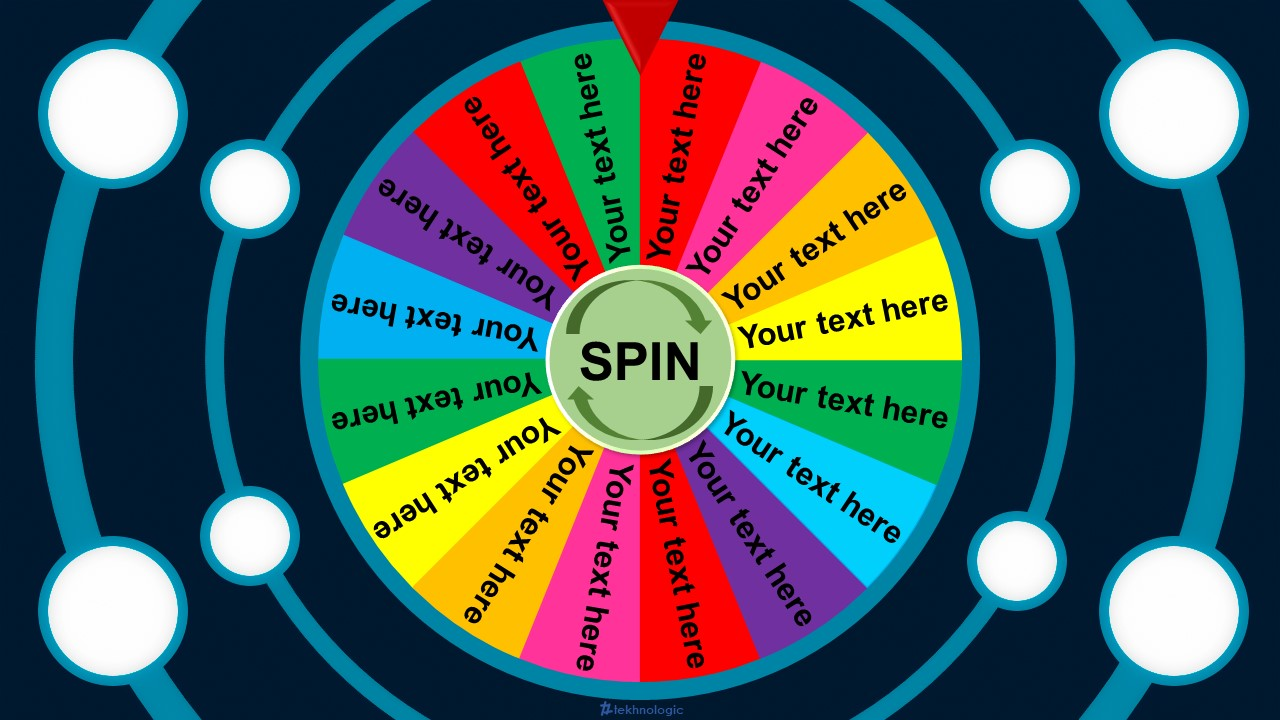
\includegraphics[width=\textwidth]{the-spinning-wheel.jpg}
            \end{figure}
        \end{column}
	\end{columns}
	\end{frame}

	\begin{frame}{Objectives}
		\begin{itemize}
		\item To explore various technologies via the process 
		\item Enhance our learning.
		\item Gain insights into how such features work. 
		\item To implement and deploy our learnings and knowledge into realising our web-app
		\item To deploy the app which provides a real-time solution to the raised issue.
		\end{itemize}
	\end{frame}

	\begin{frame}{Work Done}
		\justifying
		\begin{itemize}
		\item  Created Git Repository
		\item  Decided the tech stack
		\item  Made Weekly Plans upto 2 months
		\item  Discussed a rough idea of visual frame-work.
		\item  Learned Sphinx for Docs and Latex for ppt
		\end{itemize}
	\end{frame}


	\begin{frame}{Tech Stack}
		
    \begin{figure}
        \begin{minipage}[t]{0.2\textwidth}
            \centering
            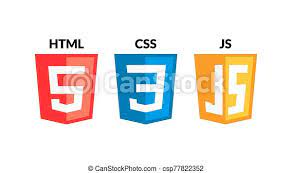
\includegraphics[width=\textwidth]{frontend.jpeg}
            \caption{Frontend}
        \end{minipage}\hfill
        \begin{minipage}[t]{0.2\textwidth}
            \centering
            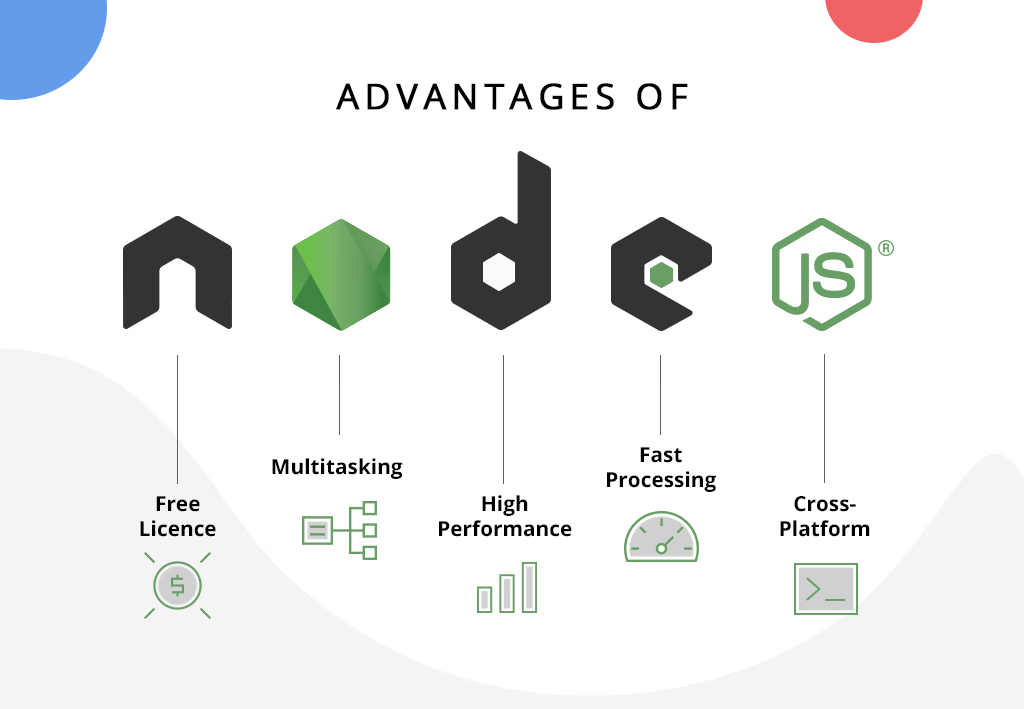
\includegraphics[width=\textwidth]{node.js_backend.png}
            \caption{Backend}
        \end{minipage}\hfill
        \begin{minipage}[t]{0.2\textwidth}
            \centering
            
\includegraphics[width=\textwidth]{mongoDB.png}
            \caption{Database}
        \end{minipage}\hfill
        \begin{minipage}[t]{0.2\textwidth}
            \centering
            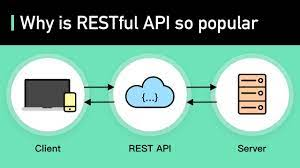
\includegraphics[width=\textwidth]{API.jpeg}
            \caption{RESTful APIs}
        \end{minipage}\hfill
        \begin{minipage}[t]{0.2\textwidth}
            \centering
            
\includegraphics[width=\textwidth]{AWS.png}
            \caption{Deployment}
        \end{minipage}
    \end{figure}
	\end{frame}

	\begin{frame}{USP}
		\justifying
		Unique Selling Proposition:
		\begin{itemize}
		\item Unmatched range of productivity features
		\item Utilizes user statistics for performance comparison
		\item Multiple productivity features		
		\item Gamification of the work by leveraging reward based human psychology
		
		\end{itemize}
	\end{frame}

	\begin{frame}{Target Audience}
	\begin{columns}
        \begin{column}{0.7\textwidth} % Adjust the width as needed
            % Content on the left side of the slide
			\begin{itemize}
			\item School and college students
			\item Competitive Exam Candidates
			\item Working professionals of all age groups
			\end{itemize}

    	\end{column}
        
    	\begin{column}{0.3\textwidth} % Adjust the width as needed
            \begin{figure}
                
\includegraphics[width=\textwidth]{student.jpeg}
            \end{figure}
    	\end{column}
    \end{columns}
	\end{frame}



	\begin{frame}{Conclusion}
		\justifying
		Hence, 'ACHIEVO' \\ 
		A web based application to help you stay
		on track and accomplish all your goals \\
	        Coming soon ! \\
		\textbf{Domain: } Web Development \\
		\textbf{Status: } Ideation \\
		
		\bigskip
		
		\Huge\textit{Thank You !}
	\end{frame}

\end{document}
